\documentclass[aspectratio=169, 14pt]{beamer}
\usepackage[utf8]{inputenc}
\usepackage[english]{babel}
\usepackage{tipa}
\usepackage{graphicx}
\usepackage{transparent}
\usepackage[ruled, lined, linesnumbered, commentsnumbered]{algorithm2e}
\usepackage{pgfplots}
\newcommand\mycommfont[1]{\small\ttfamily\textcolor{blue}{#1}}
\SetCommentSty{mycommfont}
\renewcommand{\thealgocf}{}
\usepackage{setspace}
\usepackage{tikz}
\usetikzlibrary{matrix,backgrounds}
\usetikzlibrary{arrows}
\usetikzlibrary {arrows.meta}
\usetikzlibrary{calc,shadows.blur,fit,positioning}
\usetikzlibrary{shapes.multipart,chains}
\usepackage{minted}
\usepackage{fontawesome5}
\usepackage{booktabs}
\usepackage{caption}
\usepackage{bookmark}
\usepackage{hyperref}
\hypersetup{
	colorlinks=true,
	linkcolor=blue,
	filecolor=magenta,
	urlcolor=cyan,
}
\urlstyle{same}
\usetheme{metropolis}
\metroset{block=fill}
\usecolortheme{default}
\definecolor{darkmidnightblue}{rgb}{0.0, 0.2, 0.4}
\definecolor{LightGray}{gray}{0.9}


%------------------------------------------------------------
%This block of code defines the information to appear in the
%Title page
\title[Data Structures] %optional
{Data Structures}

\subtitle{Python Crash \& Built-in Data Structures}

\author[CHEN Zhongpu] % (optional)
{CHEN Zhongpu}

\institute[] % (optional)
{
	School of Computing and Artificial Intelligence \\
	\href{mailto:zpchen@swufe.edu.cn}{zpchen@swufe.edu.cn}
}

\date[] % (optional)
{SWUFE, Fall 2022}

%End of title page configuration block
%------------------------------------------------------------


%------------------------------------------------------------
%The next block of commands puts the table of contents at the 
%beginning of each section and highlights the current section:

% \AtBeginSection[]
% {
%   \begin{frame}
%     \frametitle{Table of Contents}
%     \tableofcontents[currentsection]
%   \end{frame}
% }
%------------------------------------------------------------


\begin{document}

%The next statement creates the title page.
\frame{\titlepage}

%---------------------------------------------------------
%This block of code is for the table of contents after
%the title page
% \begin{frame}
% \frametitle{Table of Contents}
% \tableofcontents
% \end{frame}
%--------------------------------------------------------

{
	% \usebackgroundtemplate{\transparent{0.3}{\begin{picture}
	%     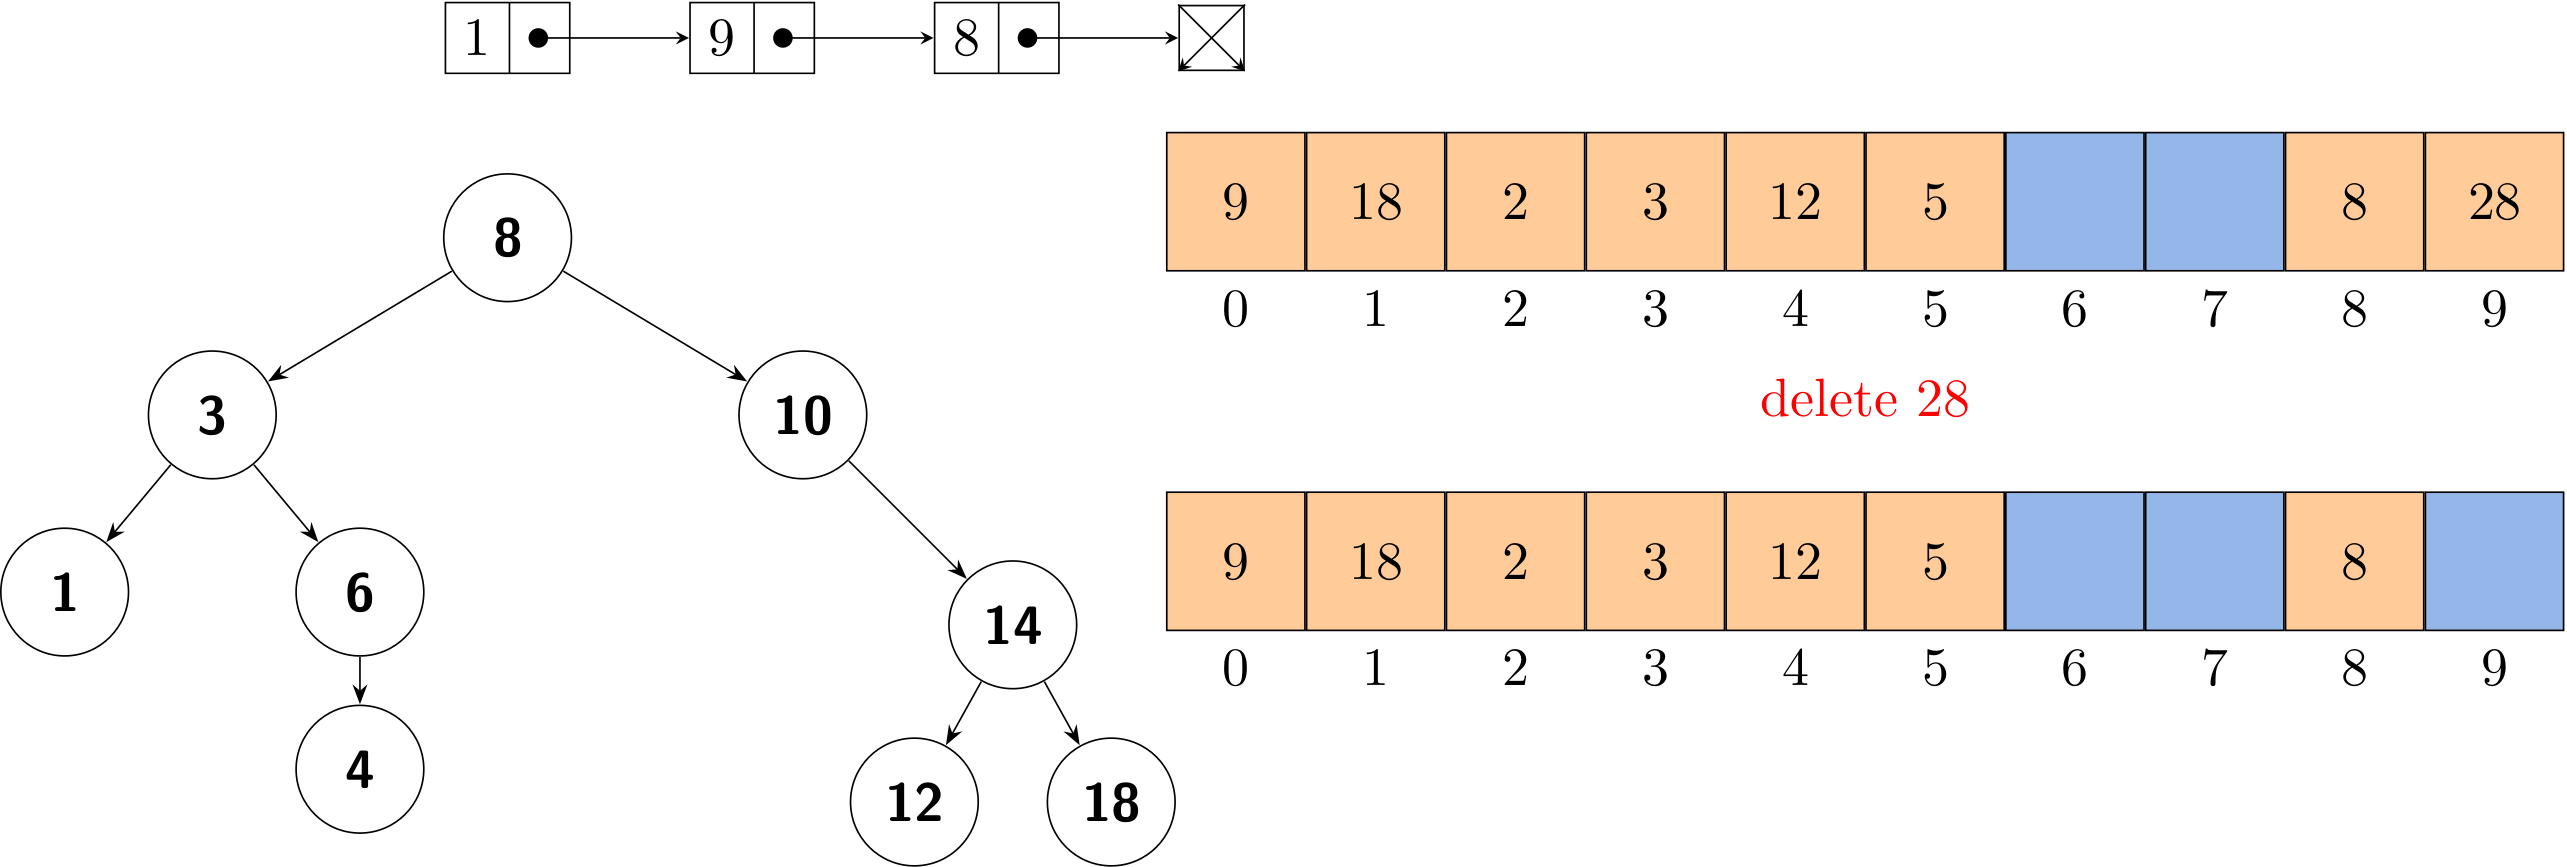
\includegraphics[height=0.7\paperheight]{cover}
	% \end{picture}    
	% }}
	\usebackgroundtemplate{
		\tikz[overlay,remember picture]
		\node[opacity=0.3, at=(current page.south east),anchor=south east, yshift=2cm,xshift=4cm] {
			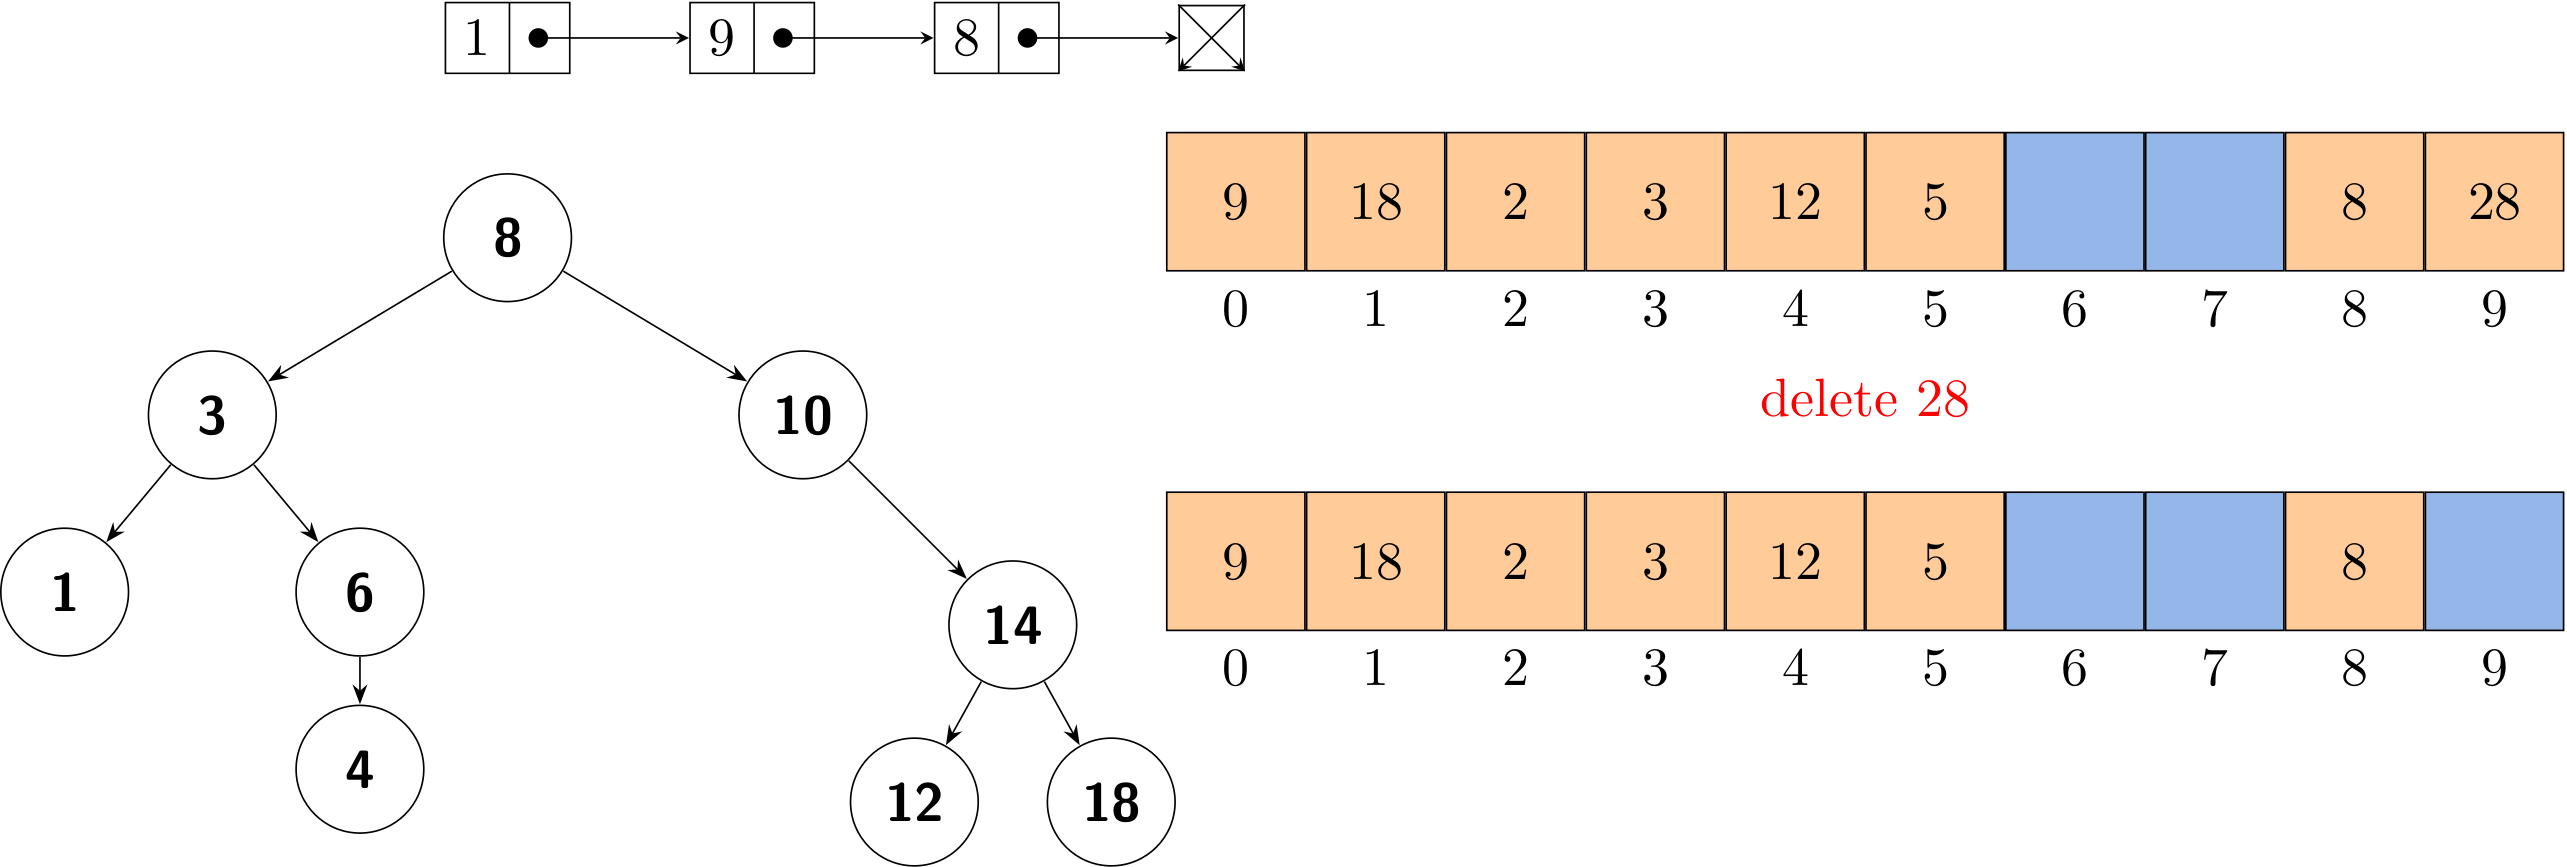
\includegraphics[height=0.6\paperheight]{cover}};
	}
	\begin{frame}
		\section{\textcolor{darkmidnightblue}{Python Crash Course}}
	\end{frame}
}

\begin{frame}
	\frametitle{How to learn Python}
	Recommended resources:

	\begin{itemize}
		\item \faIcon{python} Tutorial:\url{https://docs.python.org/3/tutorial/index.html}. Read through from Chapter 1 to Chapter 5, and Chapter 9.
		\item \faIcon{book} Book: Python Crash Course, 3rd Edition, by Eric Matthes.
		\item \faIcon{blog} Blog: \url{https://realpython.com/}
	\end{itemize}
	Yet another 8-week \href{https://github.com/ChenZhongPu/python-swufe}{course} by me. Note that \alert{class} (object-oriented programming) is not covered.
\end{frame}

\begin{frame}
	\frametitle{Overview of Python basics}
	There is no need for you to master every corner of Python. But you should be familiar with the following concepts:
	\begin{enumerate}
		\item \alert{Basic data types}: integer, float, string, boolean, list, tuple, dictionary, set
		\item \alert{Control flows}: if-else, while, for
		\item \alert{Functions}: definition, parameters, return values
		\item \alert{Classes}: definition, method, field
	\end{enumerate}
\end{frame}

\begin{frame}[fragile]

	\begin{minted}[bgcolor=LightGray]{python}
# your first Python program
print('Hello World!')
  \end{minted}

	\begin{minted}[bgcolor=LightGray]{java}
public class Main {
    public static void main(String[] args)  {
        System.out.println("Hello World!");
    }
}
  \end{minted}
\end{frame}

\begin{frame}[fragile]
	\frametitle{Variables and types}
	In Python, every variable has a type (class). Unlike Java, integers in Python have no limit in size.
	\begin{minted}[bgcolor=LightGray]{python}
# Different from Java, Python is dynamically typed,
# and you can use type() to check its type.
i = 1 
i = 3.14
i = 'hello'
i = True
i = None
  \end{minted}

\end{frame}

\begin{frame}[fragile]
	\frametitle{Math in Python}

	\begin{minted}[bgcolor=LightGray]{python}
# / always returns a float
# // is floor division
i = 1 + 2 * 2 + 9 / 2 - 9 % 2 + 9 // 2 + 9 ** 2
i = 2 > 1
j = 2 > 1 and 3 > 2
k = 1 > 2 or 3 > 2
i = not i
  \end{minted}
\end{frame}

\begin{frame}[fragile]
	\frametitle{Control flow: if}
	\begin{minted}[bgcolor=LightGray]{java}
Scanner scanner = new Scanner(System.in);
System.out.print("Input your score: ");
float score = scanner.nextFloat();
if (score >= 65) {
    System.out.println("Pass");
} else {
    System.out.println("Fail");
}
\end{minted}
\end{frame}

\begin{frame}[fragile]

	\begin{minted}[bgcolor=LightGray]{python}
score = float(input('Input your score: '))
if score >= 65:
  print('Pass')
else:
  print('Fail')
  \end{minted}
	\alert{Indentation} is important in Python! PEP8, the official guide of Python code, suggests using \alert{4 spaces} for indentation.
\end{frame}

\begin{frame}[fragile]
	Please translate the following Java code to Python:

	\begin{minted}[bgcolor=LightGray, fontsize=\small]{java}
int i = 11;
int j = 9;
if (i > j) {
    System.out.println("i is greater than j");
    if (i > 10) {
        System.out.println("i is greater than 10");
    }
} else if (i == j) {
    System.out.println("i is equal to j");
} else {
    System.out.println("i is less than j");
}
  \end{minted}
\end{frame}

\end{document}
